\documentclass[man,natbib,floatsintext]{apa6} %apa 6th edition format

% watermark for first page
% \usepackage[firstpage]{draftwatermark}
% \SetWatermarkText{In Prep}
% \SetWatermarkScale{.75}
% \SetWatermarkColor[gray]{0.88}

\usepackage{amstext,amssymb,graphicx,bm,soul,color,url,lscape,rotating,setspace,csquotes,pdflscape,rotating}
% \DeclareDelayedFloatFlavor{sidewaystable}{table}
% \DeclareDelayedFloatFlavor{sidewaysfigure}{figure}


\usepackage[space]{grffile}

% as setup by apacite, natbib puts extra spaces between the commas and semicolons in the cites. This fixes it:
\setcitestyle{citesep={;},aysep={,}}
 
% Run texcount on tex-file and write results to a file
\newcommand\wordcount{\input{wordcount.sum}}

% environment to display a page in landscape in the final pdf
\newenvironment{rotatepage}%
    {\pagebreak[4]\global\pdfpageattr\expandafter{\the\pdfpageattr/Rotate 180}}%
    {\pagebreak[4]\global\pdfpageattr\expandafter{\the\pdfpageattr/Rotate 0}}%

% commands for inserting values determined by analyses scripts.
\newcommand\shoeExplicit{290}
\newcommand\shoeIncidental{386}
\newcommand\doorExplicit{137}
\newcommand\doorIncidental{255}
\newcommand\Movie{384}
\newcommand\Relational{409}
\newcommand\Scenario{331}
\newcommand\Animacy{325}
\newcommand\Weight{322}
\newcommand\shoeExplicitAware{--}
\newcommand\shoeIncidentalAware{47}
\newcommand\doorExplicitAware{--}
\newcommand\doorIncidentalAware{43}
\newcommand\MovieAware{55}
\newcommand\RelationalAware{98}
\newcommand\ScenarioAware{32}
\newcommand\AnimacyAware{31}
\newcommand\WeightAware{31}
\newcommand\shoeExplicitIncluded{290}
\newcommand\shoeIncidentalIncluded{339}
\newcommand\doorExplicitIncluded{137}
\newcommand\doorIncidentalIncluded{212}
\newcommand\MovieIncluded{329}
\newcommand\RelationalIncluded{311}
\newcommand\ScenarioIncluded{299}
\newcommand\AnimacyIncluded{294}
\newcommand\WeightIncluded{291}
\newcommand\shoeExplicitPrec{0.46 (0.16)}
\newcommand\shoeIncidentalPrec{0.40 (0.16)}
\newcommand\doorExplicitPrec{0.47 (0.17)}
\newcommand\doorIncidentalPrec{0.47 (0.14)}
\newcommand\MoviePrec{0.38 (0.15)}
\newcommand\RelationalPrec{0.44 (0.18)}
\newcommand\ScenarioPrec{0.38 (0.14)}
\newcommand\AnimacyPrec{0.37 (0.14)}
\newcommand\WeightPrec{0.42 (0.15)}


% counter for panels of crp matrix figure
\newcounter{crppanel}

% commands for making margin notes marked with authors initials
\setlength{\marginparwidth}{30pt}
\newcommand{\mkh}[1]{\marginpar{\scriptsize \textcolor{red}{MKH: #1}}}

\title{Temporal Contiguity in Incidentally Encoded Memories} 

\author{M.\ Karl Healey}

\affiliation{Michigan State University}

\shorttitle{Contiguity with Incidental Encoding}

%\journal{???}

\authornote{I thank Mitchell Uitvlugt and Kimberly Fenn for helpful discussions. \color{red} I am grateful to James S. Nairne, Ian Neath, and an anonymous reviewer for invaluable comments during the review process.\color{black}~Correspondence concerning this article should be addressed to M. Karl Healey (khealey@msu.edu) at Michigan State University, Department of Psychology, 316 Physics Road, East Lansing, MI.
\begin{flushleft}
phone: 517-432-3107\\
Version as of \today\\
\wordcount words (Approximate due to use of \LaTeX)
\end{flushleft}
}
\setstcolor{red}
\abstract{Thinking of one event often triggers recall of other events experienced nearby in time. This Temporal Contiguity Effect effect has been extensively documented in laboratory list learning tasks, but its source is debated. Is it due to task-general automatic processes that operate whenever new memories are formed? Or is it due to task-specific encoding strategies that operate only during deliberate rote learning? I test these theories by looking for the Temporal Contiguity Effect when there is no intent to memorize, as is often the case outside the laboratory. Experiments 1 and 2 confirm that temporal contiguity can be \st{absent} \color{red} dramatically reduced\color{black}~under incidental encoding. \st{Experiment 3 shows that it is not the intent to memorize per se, but rather how subjects process information while incidentally learning it that generates temporal contiguity.} \color{red}Experiments 3 and 4 show that although the effect is reduced, it is not eliminated---some temporal information is encoded incidentally and is used to guide memory search during both free recall and serial recall. These results show that contiguity is not an artifact of strategy, but they also challenge models that posit a strong link between successful memory encoding and contiguity.
\color{black}}
\keywords{episodic memory; free recall; temporal contiguity}

\begin{document}
\maketitle
\label{TODO-1}
% Recalling one event tends to trigger recall of other events experienced nearby in time \citep{HealKaha17}. This Temporal Contiguity Effect (TCE) manifests in many tasks \citep{DaviEtal08,SchwEtal05}. For example, in free recall, you study words presented serially and recall them in any order. After recalling the word studied in the $5^{th}$ serial position, your next recall is much more likely to be from the $6^{th}$ or $4^{th}$ position than more distant positions \citep{Kaha96}. 

% The TCE has shaped theories of the testing effect \citep{KarpEtal14}, directed forgetting \citep{SahaEtal13}, retrieval induced forgetting \citep{KlieBaum16}, childhood development \citep{JarroEtal15}, cognitive aging \citep{WahlHuff15,HealKaha15}, event segmentation \citep{EzzyDava14}, time estimation \citep{SahaSmit13}, and even perception \citep{TurkEtal12}. Yet, we still do not know which cognitive processes create the effect \citep{HealKaha17}. Here, we will consider two classes of explanation. First, that the TCE arises from control processes that are only engaged when we are deliberately forming new memories. Second, that the TCE arises from processes that the memory system automatically engages whenever new memories are formed, be it deliberately or incidentally. 
\color{red}
Recalling one event tends to trigger recall of other events experienced nearby in time \citep[for a review, see][]{HealKaha17}. Although this Temporal Contiguity Effect (TCE) manifests in many memory tasks \citep{DaviEtal08,SchwEtal05}, it is most readily observed in free recall where participants study a list of words presented serially and then try to recall the words. Despite the fact that participants are free to recall the items in any order, the order of recall tends to recapitulate the order of study \citep{Murd74,Post71,Post72,Kaha96}. %For example, \citet[][p. 202]{Murd74} observed that, after quickly outputting the most recent items, participants tend to jump to an earlier point in the list and then recapitulate the presentation order, with a bias to do so in the forward direction.

The TCE can be illustrated by computing the probability of successively recalling items as a function of their distance, or lag, from each other in the study list \citep{Kaha96}. For example, if after recalling the word studied in the $5^{th}$ serial position, your next recall is the word from the $6^{th}$ serial position, you have made a $lag=+1$ transition. If instead you transitioned from recall of the $5^{th}$ serial position to the $3^{rd}$ position, you have made a $lag=-2$ transition. For each value of lag, the conditional-response probability (CRP) is computed by dividing the number of times a transition of that lag was \emph{actually} made by the number of times it \emph{could} have been made \citep[e.g., if you have just recalled the last item in the list, it is not possible to make a $lag=+1$ transition. Transitions to already recalled items are also excluded from the counts as subjects rarely repeat items;][]{Kaha96}. The lag-CRP typically is highest for $lag=+1$ and $-1$ (but with a forward asymmetry) and decreases sharply for larger absolute values of lag. That is, memory search tends to transition between words that were studied nearby in time.

The TCE has shaped theories of the testing effect \citep{KarpEtal14}, directed forgetting \citep{SahaEtal13}, retrieval induced forgetting \citep{KlieBaum16}, childhood development \citep{JarroEtal15}, cognitive aging \citep{WahlHuff15,HealKaha15}, event segmentation \citep{EzzyDava14}, time estimation \citep{SahaSmit13}, and even perception \citep{TurkEtal12}. Moreover, out of several of factors that influence free recall (i.e., primacy, recency, and semantic similarity), the magnitude of the TCE has been found to be the most predictive of overall memory ability \citep{SedeEtal10,SpilUnsw11} and general intellectual ability \citep{HealEtal14}.

Yet, we still do not know which cognitive mechanisms generate the TCE \citep{HealKaha17}. Here, I will consider two classes of explanation. First, that the TCE arises from task-specific mechanisms that are only engaged when we are deliberately studying a serially presented list. Second, that the TCE arises from task-general mechanisms that the memory system automatically engages whenever new memories are formed.% be it deliberately or incidentally. 



\label{TODO-2}   
\subsection{Task-Specific Mechanisms}
Control processes \citep{LehmMalm13,AtkiShif68} allow us to strategically process information during memory encoding, maximizing recall \citep[e.g.,][]{Unsw16,DelaKnow05}. Some work suggests that the TCE arises from such task-specific strategies, implemented by control processes to handle the idiosyncratic demands of laboratory tasks \citep{Hint16}. In other words, because laboratory tasks require subjects to do something they do not usually do (e.g., learn lists of largely unrelated words), they are forced to devise novel strategies to adapt to the peculiarities of the task. Such task-specific strategies, rather than task-independent memory mechanisms, could account for the contiguity effect.

As an example, the standard free recall task may encourage subjects to adopt the strategy of linking successive list items together to tell a story \citep{DelaKnow05}. Another example of a task-specific contiguity-generating mechanism is the method of loci, in which the list items are associated with a pre-memorized sequence of locations. Both of these strategies require subjects to pay attention to the order of presentation and recapitulate it during recall. Thus, both would produce a TCE.

But critically, subjects deploy these contiguity-generating strategies only because they happen to be well-suited to the specifics of the task. If the specifics of the task change, subjects may adopt different strategies, and these new strategies may not generate contiguity.
If the strategies are the only mechanism generating contiguity, any change in the specifics of the task that causes subjects to abandon contiguity-generating strategies should eliminate the TCE entirely. The most decisive test of this prediction is to have participants process the list under incidental encoding conditions, which should prevent adoption of any deliberate encoding strategy, and then complete a surprise free recall test \citep{Hint16}.

\subsection{Task-General Mechanisms}
Participants obviously adopt task-specific strategies. And these strategies doubtlessly contribute to the TCE. But task-specific strategies many not be the only mechanisms that generate the TCE.\footnote{Indeed, \citet{Hint16} suggests that in addition to engaging deliberate contiguity-generating strategies, subjects might also automatically notice similarities among temporally proximate items and therefore remember them together at recall.} Many theories of episodic memory propose \emph{task-general} mechanisms that automatically encode information about the temporal proximity of events when forming episodic memories, even if no specific encoding strategy is adopted. If these models are correct, a residual TCE should remain even after removing any impetus to engage encoding strategies.

As an example, some theories assume that new events form associations to a representation of time \citep{HowaEtal14a,BrowEtal07}. This allows recall of one event to trigger recall of temporally adjacent events via associations to adjacent temporal representations. These theories assume time is directly encoded by the memory system, but this is not the only way the memory system might automatically encode information about presentation order. Other theories assume that events experienced close together in time become associated, not with a temporal representation, but with similar states of a drifting mental context representation \citep{PolyEtal09,LohnEtal14,McGe32}. This allows recall of one word to trigger recall of a word studied nearby in time via associations to a common state of mental context. Either of these mechanisms would provide the necessary ingredients to produce a TCE during free recall. 

However, these encoding mechanisms are assumed to support memory in a range of situations and not just during laboratory list learning tasks. If the specifics of the task change, subjects may adopt different strategies, but they must still rely on the fundamental mechanisms of the memory system. Therefore, changes in specifics of the task might modulate the magnitude of the TCE by changing the contribution of context-generating strategies, but they should not eliminate the TCE entirely. Thus, these theories would predict that a residual TCE should be observed even under incidental encoding.

\subsection{Incidental Encoding of Temporal Order}
The task-specific and task-general perspectives make competing predictions about the influence of removing the intention to encode on the size of the TCE. The literature on incidental encoding provides some data relevant to these predictions, but scholars' interpretations of these findings are mixed. 

\citet{GlenBrad79} tested for incidental encoding of temporal associations by having subjects repeat a pair of words while trying to retain digits for 1, 5, or 10 seconds. After 81 such trials, subjects were given two surprise memory tests for the words. The first was an item recognition test (i.e., was the probe seen before); the second was either a cued recall test (given one word from a pair, recall the other) or a pair recognition test (discriminate intact from mismatched pairs). Performance was above chance on the item and pair recognition tests but was very low on the cued recall test, suggesting participants had limited access to information about which words appeared together. A second experiment also found very low cued recall performance but above chance performance on an associative matching test. \citet{BradGlen83} replicated their earlier findings and added many control conditions, including a ``sheer contiguity'' condition in which the words were not presented simultaneously as in the previous experiment but merely in close temporal proximity (as is the case in free recall). In this condition, performance on the associative recognition task was not above chance. \citet[][p. 665]{BradGlen83} concluded ``that sheer temporal contiguity, that is, adjacency of processing, is not sufficient to produce the associations observed in these experiments.''

Data from \citet{Nair91, Nair90b} suggest a different conclusion. In several studies, participants viewed lists of serially presented words under the guise of a rating task. This incidental encoding task was followed by a surprise order reconstruction task in which subjects were shown the words and had to reconstruct their order. They could do this with considerable accuracy, even when they were shown multiple lists and required to place each word in both its correct list and its correct within-list position \citep{Nair91}. Moreover, even when participants made a mistake on the reconstruction task, the errors were not random. Instead, order errors following incidental encoding tended to take the form of putting items in positions adjacent to the correct ones, much as they do after explicit encoding \citep{Heal74}. This work suggests that subjects have relatively easy access to temporal information. 

But other work shows that even after explicitly studying a list for a recognition task, subjects preform poorly if they are instead given a surprise spacing judgment task, which requires them to guess the lag that separated pairs of words from the original list, unless the words in the pair were semantically related \citep{HintEtal75,HintBloc73}. These results have been taken as evidence that temporal information is only encoded when subjects notice semantic similarities among items in the list \citep[i.e., study phase retreival]{HintEtal75,HintBloc73,Hint16}.

\label{TODO-4}
In all of these studies, the test directly asked participants to access information about temporal order. But being explicitly aware of the order of a list and being able to report it is not the same thing as allowing temporal information to influence memory search during free recall. It is possible that participants could have the temporal information needed to complete an ordering task but fail to use that information to guide a free memory search. Or vise versa, participants could have difficulty explicitly recalling order yet still implicitly access temporal information to guide memory search. In other words, do participants spontaneously use incidentally encoded temporal information to produce a TCE in free recall? 

The most direct test for a TCE during free recall after incidental encoding comes from a series of studies reported by \citet{NairEtal17}, which were designed to investigate the causes of the survival processing effect \citep{NairEtal07}. In the first experiment, subjects completed a survival processing task: subjects viewed a list of items and for each rated its relevance to a survival (or control) scenario. There was a surprise free recall test approximately two minutes after the end of the list. Despite recalling many words (approximately 45\% accuracy across conditions), the TCE was not significantly above chance. A second experiment replicated this null TCE using a different processing task as a control to the survival processing task. \citet{NairEtal17} included a third experiment that used the same incidental encoding procedure as their first two experiments, but instead of a free recall test, subjects were provided with all of the words from the list and asked to reconstruct the order. This direct test of order memory did reveal a robust TCE in both the survival processing and the control condition. This finding suggests that subjects may be incidentally encoding information about temporal order but failing to spontaneously use it during free recall.

If incidental encoding really does eliminate the TCE in free recall, it would constitute strong evidence against many models of the effect \citep[e.g.,][]{LohnEtal14,HealKaha17}. However, further investigation is warranted before concluding that incidental encoding will always eliminate the TCE. Because the \citet{NairEtal17} study was about survival processing and not the influence of intent to encode on the TCE, it did not include an explicit encoding control condition and included some features, other than intent to encode, that are known to influence the TCE. In particular, it used a single, relatively long list (32 items). The TCE is known to be modestly reduced by both lack of task experience and long lists \citep{HealKaha17}. It is possible that aspects of the task other than incidental encoding contributed to the null TCE. Therefore, Experiment 1 directly compares the TCE in \label{TODO-3} free recall after explicit versus incidental encoding.
\color{black}

\section{Experiment 1}
\st{As an initial experiment, we attempted to conceptually replicate the Nairne et al. (2017) finding of no TCE under incidental encoding. To facilitate comparison with other studies in the TCE literature, the experiment included an explicit encoding control condition and used standard free recall methods and a commonly used encoding task.}
\color{red}
The goal of the first experiment was to assess whether incidental encoding reduces the TCE relative to explicit encoding. All subjects viewed a list of words presented one at a time and made a simple judgment about each. Participants in the Explicit condition were expecting a memory test; participants in the Incidental condition were \emph{not} expecting a memory test.  After the last item, all subjects were asked to recall as many of the words as they could, in any order. 
\color{black}

\section{Method}

% setup some commands to make changing text from study to study easy
\newcommand\listlength{16} % words per list 
\newcommand\presrate{4 seconds} % time per word
\newcommand\isi{1 second} %
\newcommand\DFRDelay{16 second} % length of distractor at end of study
\newcommand\recalltime{75 seconds} % time to recall
\newcommand\totalss{XX}
\newcommand\totalexcluded{XX}



\subsection{Data Sharing}All data analyzed in this report are freely available on the author's website (https://cbcc.psy.msu.edu/data/Heal16implicit.csv).

\subsection{Subjects}

Given that manipulating encoding intention might reduce, but not eliminate, the TCE, it is critical to have sufficient power to detect small effects. \citet{SedeEtal10} reported a meta-analysis of the TCE in explicit encoding studies; power calculations revealed that a sample size of 143 per condition would provide a $1-\beta$ power of 0.95 to detect (via a 1-tailed 1-sample t-test) an effect one fifth the size of the average effect they reported.
% here is how to get the SD: ((.614-.5)/31.2)*np.sqrt(510)
In order to collect enough data to meet or exceed this sample size in the Incidental conditions, subjects for all of the experiments reported here were recruited using Amazon's Mechanical Turk, a crowdsourcing website that allows for efficient collection of large volumes of high-quality data. Subjects were paid \$1.00 for participating (a rate of roughly \$10 / hr).~\label{TODO-10} \color{red}The demographics of the Mechanical Turk community have been described elsewhere \cite[approximately 55\% female with a mean age of 32;][]{MasoSuri12}. Due to time constraints, no demographic information was collected from participants for Experiments 1--3. Demographic information was collected in Experiment 4 (subjects in that experiment were overwhelmingly native English speakers with a high school education or a college degree; see that study's Method section for details). \color{black}

Subjects in the Incidental conditions were excluded from analysis if they reported in a post-experiment questionnaire that they suspected their memory would be tested while they were preforming the Incidental encoding task. The final analyzed sample was composed of \shoeExplicitIncluded~in the Explicit condition and \shoeIncidentalIncluded~in the Incidental condition. Table~\ref{sampsize_table} shows the total number of included and excluded subjects for each experiment.

\subsection{Procedure}
All subjects completed two free recall lists \st{(only the first of which is analyzed here)}. Each list was composed of \listlength~words drawn randomly from a pool of 1638 words, with the constraint that no word was used more than once for a given subject. Words were presented one at a time on the subject's computer screen for \presrate. This presentation rate was deliberately chosen to be slightly faster than the 5 seconds per word used by \citet{NairEtal17} to reduce the amount of ``free time'' subjects have between making the judgment and the presentation of the next word.
There was an inter-stimulus interval of \isi~between word presentations during which a fixation cross was displayed in the same location where the words appeared. The final word of each list was followed by a \DFRDelay~distractor period during which subjects answered math problems of the form $A+B+C=$~?, where $A$, $B$, and $C$ were positive, single-digit integers, though the answer could have been one or two digits. Subjects typed their answers to the math problems in a text box and pressed enter to submit. Upon pressing enter, a new math problem and a new blank text box appeared. Subjects were instructed to ``Try to solve as many problems as you can without sacrificing accuracy. The task will automatically advance when the time is up.''.

Following the math distractor task, subjects in both conditions were asked to recall as many items as possible from the preceding list, in any order. Subjects typed each recalled word in a text box and pressed enter to submit the word. Upon pressing enter, the word disappeared and a new blank text box appeared such that subjects could not see their prior responses. Subjects were given \recalltime~to recall as many words as they could. To ensure subjects noticed that the recall period had begun (e.g., were not looking at the keyboard and typing their answer from the final math problem), a red screen was flashed for 500 ms before the recall instructions were displayed and the recall text box did not begin accepting input for a further 500 ms. Therefore, including the math distractor, there was a total delay of $16+0.5+0.5=17$ seconds between the end of the study period and the beginning of the recall period. A spell-checking algorithm (described in the Supplemental Materials) checked subjects' typed responses for typos and scored their recall accuracy.


% TODO: check these aginst the values in the pandas tables in alan_funct E4_sample_size_table by stopping in debugger
% sample size table
\begin{table}
\caption{Sample sizes, exclusions, and recall probability by condition.}
\label{sampsize_table}
\begin{tabular}{llcccc}
\thickline
    Exp & Condition & $n$ Included & $n$ Excluded  & Recall  \\
     &  &  &  (aware) & Prob. (SD) \\
  Exp1  \\
  & Explicit &  \shoeExplicitIncluded & \shoeExplicitAware & \shoeExplicitPrec \\
  & Incidental &  \shoeIncidentalIncluded & \shoeIncidentalAware & \shoeIncidentalPrec \\
    Exp2  \\
  & Explicit &  \doorExplicitIncluded & \doorExplicitAware & \doorExplicitPrec \\
  & Incidental &  \doorIncidentalIncluded & \doorIncidentalAware & \doorIncidentalPrec \\
  Exp3  \\
  & Weight &  \WeightIncluded & \WeightAware & \WeightPrec \\
  & Animacy &  \AnimacyIncluded & \AnimacyAware & \AnimacyPrec \\
  & Moving Scenario &  \ScenarioIncluded & \ScenarioAware & \ScenarioPrec \\
  & Movie  &  \MovieIncluded & \MovieAware & \MoviePrec \\
  & Relational &  \RelationalIncluded & \RelationalAware & \RelationalPrec \\
  Exp4  \\
  & Varying--Free &  \VaryingFreeIncluded & \VaryingFreeAware & \VaryingFreePrec \\
  & Constant--Free &  \ConstantFreeIncluded & \ConstantFreeAware & \ConstantFreePrec \\
  & Constant--Serial &  \ConstantSerialIncluded & \ConstantSerialAware & \ConstantSerialPrec \\
\hline
\end{tabular}
\end{table}

\subsubsection{Encoding Instructions Manipulation} Subjects were randomly assigned to either the Incidental condition or the Explicit condition. Prior to seeing the first list, subjects in both conditions were told that they would see a series of words and would make a simple judgment about each one (i.e., Would it fit in a shoebox?). The exact instructions depended on the condition. In the Explicit condition, subjects were given standard free recall instructions that described the size judgment task but emphasized memory. In the Incidental condition, subjects were given instructions only for the size judgment task and memory was never mentioned. Because the wording of the instructions are integral to the intent manipulation, they are reproduced exactly in the Supplementary Materials.

\subsubsection{Shoebox Task} In both conditions, subjects were asked to make a size judgment about each word while it was present on the screen. Specifically, they were asked  to judge if the word referred to an object that could fit into a shoebox. To allow for the same yes/no response across all conditions and all experiments, subjects were asked to indicate if the judgment was easy to make under the guise of norming the items for a later study. See the Supplemental Materials for the exact task instructions as well as measures taken to ensure subjects understood the task instructions.

\subsection{Quantifying the Temporal Contiguity Effect} \st{The TCE is most often examined using a \textit{lag conditional-response probability} function or lag-CRP. The lag-CRP gives the probability that recall of an item studied in position $i$ of a study list will be followed by recall of an item studied in position $i+lag$. For example, if recall of the item from position 5 was followed by recall of the item from position 6 the lag would be 1. If, however, it was followed by recall of the item from position 3, the lag would be -2. For each lag, the CRP is computed by dividing the number of times a transition of that lag was \emph{actually} made by the number of times it \emph{could} have been made (e.g., it could not have been made if the item $i+lag$ was already recalled; Kahana, 1996). The lag-CRP is typically highest for lags 1 and -1 and decreases sharply for larger absolute values of lag. If the TCE is reduced under incidental encoding conditions, the lag-CRP should be flatter.}

The lag-CRP provides a visual representation of the TCE, but for several reasons it is useful to have a single number that quantifies the size of the effect. \st{When evaluating the size of the TCE,} \color{red}First,\color{black}~it is important to take into account the fact that the likelihood of successful recall is not random with respect to serial position (e.g., there are primacy and recency effects, or more generally autocorrelations in goodness of encoding), which can artificially increase the size of the TCE\color{red}~by disproportionately increasing the number of possible ways one can make short-lag transitions \citep{HealKaha17,Hint16}. Second, the lag-CRP can also \emph{underestimate} the size of the TCE in some cases. Imagine a subject who successfully encodes only three items: those from serial positions 3, 8, and 16. Even if this participant's memory search was guided by only temporal associations and they recalled the three items in perfect temporal order, they could not possibly make any transition shorter than $lag=|5|$.

To address these confounds between recall accuracy and the TCE, I combined the \emph{temporal factor score} \citep{SedeEtal10,PolyEtal09} with a shuffling procedure\color{black}. The temporal factor score is computed by ranking the absolute value of the lag of each actual transition with respect to the absolute values of the lags of all transitions that were possible at that time, which provides a percentile score for each transition. Averaging these percentile scores across all of a subject's transitions provides the temporal factor score.
\st{The size of this artificial TCE can be measured} \color{red}Temporal factor scores can be influenced by confounds with recall accuracy, but this influence can be estimated and removed \color{black} by taking the items which a subject actually recalled for a given list, randomly shuffling (i.e., permuting) the order of recalls, and recomputing the temporal factor score. Repeating this permutation procedure many times provides a distribution of the temporal factor score expected if recall transitions are completely random with respect to lag \citep{HealKaha17}. 

This logic was used to provide a corrected measure of the TCE for each participant. For each list, the temporal factor score was computed for the actual recall sequence and for 10,000 random permutations of the sequence. The actual temporal factor score was then converted into a z-score, z(TCE), by subtracting the permutation distribution's mean and dividing by its standard deviation.  \color{red}\label{TCEex} For example, imagine that a participant recalled three words: those from serial positions 6, 5, and 8, in that order. The actual temporal factor score for that recall sequence is 0.84. We would build a distribution of the temporal factor score expected by chance by taking this recall sequence and randomly shuffling it. For example, rearranging the sequence to 5, 6, 8 gives a temporal factor score of 0.92. Rearranging the sequence to 6, 8, 5 gives a temporal factor score of 0.77. Doing this for all six possible permutations of the sequence, we find that the distribution of possible temporal factor scores has a mean of 0.83 and a standard deviation of 0.06, which gives our observed temporal factor score a $z(TCE)=\frac{0.84-.83}{.06}=0.17$. \color{black}~In the absence of a true TCE, the expected value of z(TCE) is zero, so we can test for a TCE by determining if the across-subject average of z(TCE) is significantly above zero. %\color{red} Note that this procedure is conservative in that it reduces the chance of a false positive in detecting a TCE at the cost that it may underestimate the true size of the TCE. This is because the shuffling procedure assumes that the TCE influences only the order in which successfully recalled items are output, and does not influence which items successfully recalled.\color{black}



\section{Results and Discussion}

Figure~\ref{e1_l1_crp} shows the lag-CRP and corrected temporal factor scores for the Explicit and Incidental conditions. The Explicit condition shows a clear TCE: the lag-CRP is highest for short lags (i.e., $|lag|=1$) and decreases for larger lags. Moreover, the 95\% confidence interval on the z(TCE) lies well above zero. By contrast, the Incidental condition shows no evidence of a TCE: the lag-CRP is nearly flat and the 95\% confidence interval on the z(TCE) includes zero. \color{red} These results show that removing the intent to encode can reduce the magnitude of the TCE to the point that it is statistically indistinguishable from zero.\color{black}  \st{These results suggest that removing the intent to encode can eliminate the TCE.}



%#####################
%####### E1 CRP ######
%#####################
\newcommand\paneltext{(A) Lag-conditional response probability functions. Error bars are bootstrapped within-subject 95\% confidence intervals. (B) The average z(TCE).  Error bars are bootstrapped between-subject 95\% confidence intervals. z(TCE) for a given subject is computed as follows: An observed temporal factor score was computed as the average percentile ranking the temporal lag of each actual transition in the recall sequence with respect to the lags of all transitions that were possible at that time. To determine the temporal factor score expected by chance, a permutation distribution was created by randomly shuffling the order of recalls within the sequence 10,000 times and computing a temporal factor score for each shuffling. The reported value, z(TCE), is z-score of the observed temporal factor score within the permutation distribution.}
\begin{figure}
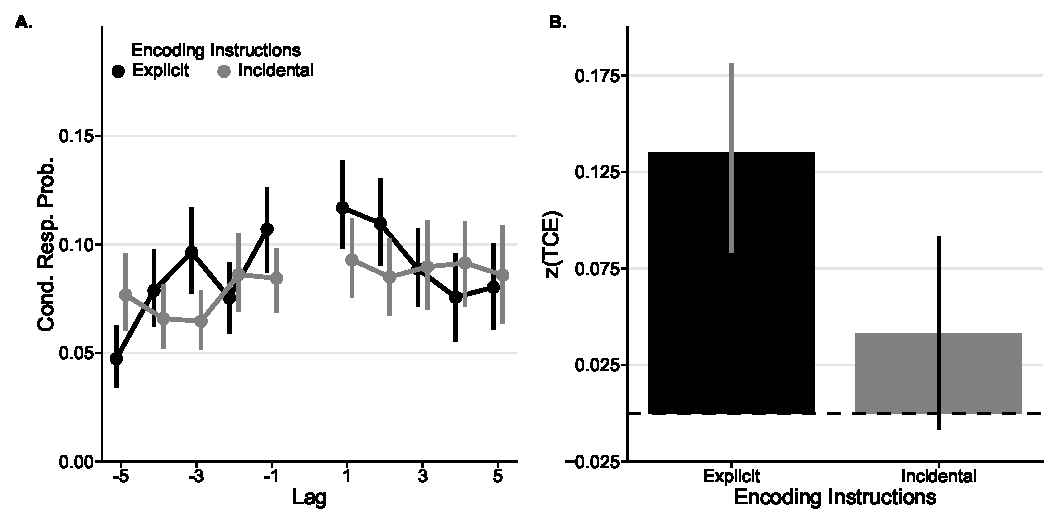
\includegraphics{figures/E1_crp_list1.pdf}
\caption{The temporal contiguity effect (TCE) on the first list under Explicit versus Incidental encoding using the Shoebox Task (Experiment 1). \paneltext}
\label{e1_l1_crp}
\end{figure}





\color{red}
\label{TODO-5}
It is notable that even in the Explicit condition, the TCE was small and more symmetric than the TCEs reported in most previous work. Across a range of variations of the free recall task, the lag-CRP typically peaks at about 0.3--0.5 \citep{HealKaha17} compared to approximately 0.12 for the current Explicit condition. The critical difference is likely amount of task experience. In a multi-list explicit encoding study, \citet{HealKaha17} found that on a participant's very first list, the lag-CRP peaked at approximately 0.15, but on the twelfth list, it peaked at 0.3. Figure~\ref{e1_l2_crp} shows the TCE for the second list in the current study. In both conditions, the z(TCE) is numerically higher than on the first list, but not significantly so ($p=0.07$ and $p=0.32$ for the Incidental and Explicit conditions respectively)\label{t1}. Moreover, the TCE is still lower in the Incidental than the Explicit condition, perhaps reflecting that the Explicit condition are profiting from the encoding practice they gained on the first list. These findings would be difficult to account for with most existing models, because they have no mechanism to simulate practice or otherwise allow contiguity to change dramatically with task experience.

%#####################
%####### E1l2 CRP ####
%#####################
\begin{figure}
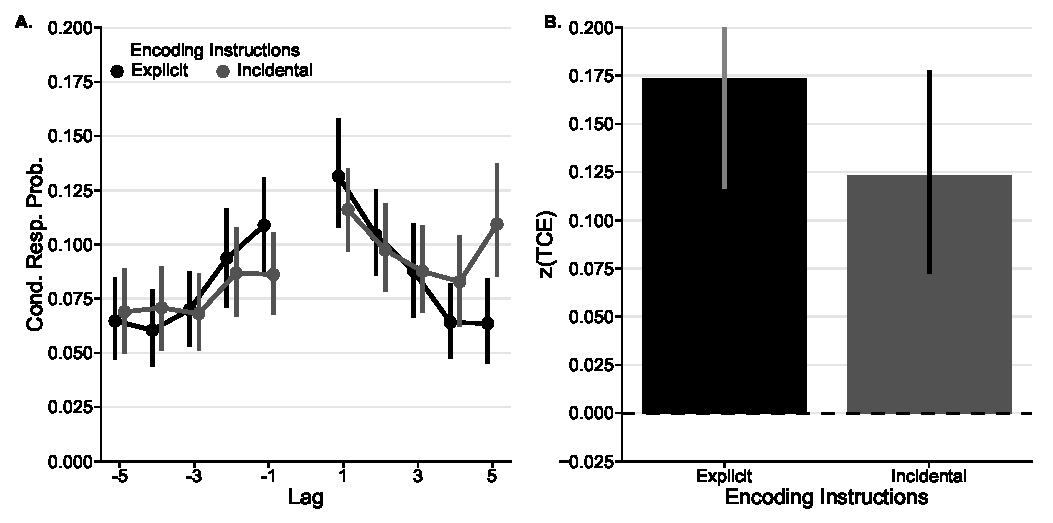
\includegraphics{figures/E1_crp_list2.pdf}
\caption{The temporal contiguity effect (TCE) on the second list under Explicit versus Incidental encoding using the Shoebox Task (Experiment 1). \paneltext}
\label{e1_l2_crp}
\end{figure}

\color{black}


\color{red}
\label{TODO-6}
Although the TCE is our main focus, \label{SPCtalk} examining other aspects of recall dynamics may help shed light on why the TCE varies across conditions. Overall recall probability (Table~\ref{sampsize_table}) was lower in the Incidental than the Explicit condition. This is largely attributable to participants in the Incidental condition recalling fewer items from early serial positions as can be seen in the serial position curves (SPC) in Figure~\ref{e1_l1_spc}A. Both groups show considerable recency despite the incidental encoding and a delayed test \citep[for a similar findings, see][]{MarsWerd72,Neat93,GlenEtal80}.

%#####################
%####### E1l1 SPC ####
%#####################
\newcommand\spcpaneltext{All error bars are bootstrapped within-subject 95\% confidence intervals.}
\begin{figure}
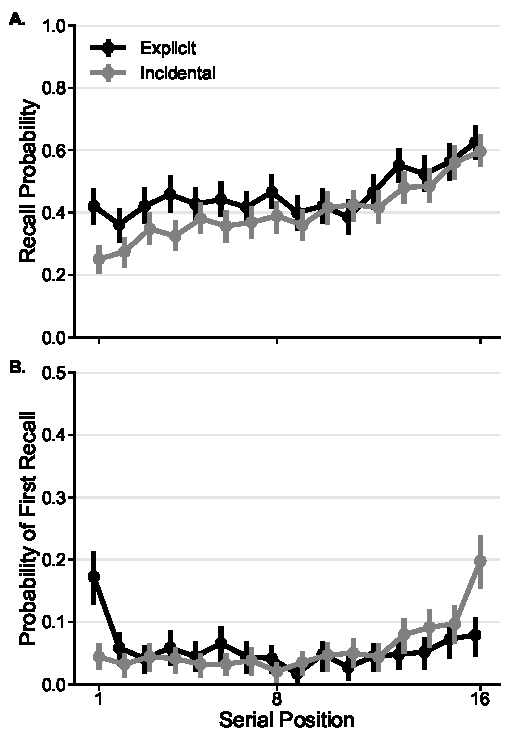
\includegraphics{figures/E1_spc_list1.pdf}
\caption{(A) Serial position curves and (B) probability of first recall curves on the first list under Explicit versus Incidental encoding using the Shoebox Task (Experiment 1). \spcpaneltext}
\label{e1_l1_spc}
\end{figure}

How participants initiate recall, as revealed by probability of first recall (PFR) curves (Figure~\ref{e1_l2_spc}B), is also informative. In delayed free recall tasks, participants typically initiate recall by first retrieving an item from near the beginning of the list \citep[i.e., they focus first on primacy items;][]{HowaKaha99}. Participants in the Explicit condition showed this typical pattern, but participants in the Incidental condition showed the opposite pattern of focusing first on recency items (Figure~\ref{e1_l1_spc}B), which is more typical of immediate recall \citep{Hoga75}. On the second list, when everyone expected a memory test, these group differences in recall initiation and accuracy were eliminated.

These differences in recall dynamics between incidental and explicit encoding may be due to removing the impetus to rehearse \citep{MarsWerd72,Neat93,GlenEtal80}, which is known to increase primacy by effectively increasing the  functional serial position of early list items \citep{Rund71,BrodMurd77,TanWard00}. But what about the TCE? Rehearsal could increase the TCE by causing subjects to hold adjacent items in mind at the same time \citep{Hint16}. Although the TCE has been found under conditions designed to minimize rehearsal \citep{HowaKaha99}, reduced rehearsal may be one factor contributing to a diminished TCE under incidental encoding.

%#####################
%####### E1l2 SPC ####
%#####################
\begin{figure}
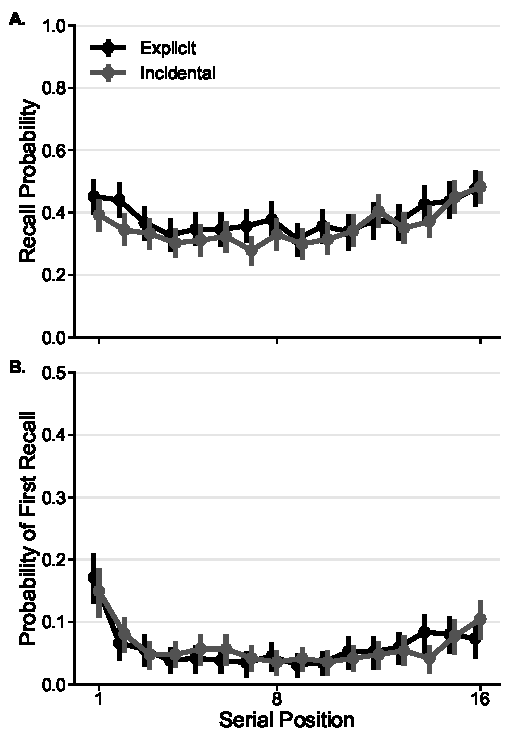
\includegraphics{figures/E1_spc_list2.pdf}
\caption{(A) Serial position curves and (B) probability of first recall curves on the second list under Explicit versus Incidental encoding using the Shoebox Task (Experiment 1). \spcpaneltext}
\label{e1_l2_spc}
\end{figure}

In summary, Experiment 1 directly compared Explicit and Incidental encoding conditions and found that removing the intent to encode dramatically reduced the TCE. \color{black} But because the TCE has proven to be so robust in previous studies \citep{HealKaha17}, I attempt to replicate the finding in Experiment 2 using a slightly different processing task.




\section{Experiment 2}
\section{Method}

The methods were identical to those used in Experiment 1 except for the judgment task instructions (see Table 1 for sample size information).
The processing required by the Shoebox Task from Experiment 1 is quite simple. So simple that one could argue it is  ineffective at forming strong memories \label{newcite}\citep{EaglLeit64}, which may artificially reduce the TCE. Therefore, I wanted to retain the basic task of judging size while increasing memory performance in the Incidental condition. That is, can processing that promotes memory do so without producing substantial contiguity? Mental imagery and self-referential processing are two effective ways to improve memory. Thus, the Front Door Judgment Task asked subjects to imagine trying to move the object referred to by each item through the front door of their house and decide whether or not it would be possible:~\label{newinst}\color{red}``Specifically, for each word, you will think of the object it refers to and try to imagining yourself moving that object through the front door of your home. Ask yourself if the object would successfully fit through your front door.''\color{black}~Again, subjects were asked to indicate if this judgment was easy or difficult to make by pressing ``Y'' or ``N''. See the Supplemental Materials for the exact task instructions.

\section{Results and Discussion}
As predicted, the Front Door Task substantially improved memory accuracy in the Incidental condition. In fact, probability of recall was equal in the Explicit and Incidental conditions (Table 1) \color{red} and the differences in serial position and probability first recall curves were reduced (Figure~\ref{e2_l1_spc}). Together, these findings suggest factors that influence memory accuracy, like rehearsal, played less of a role in in producing differences between the Explicit and Incidental conditions in this experiment.

%#####################
%####### E2l1 spc ####
%#####################
\begin{figure}
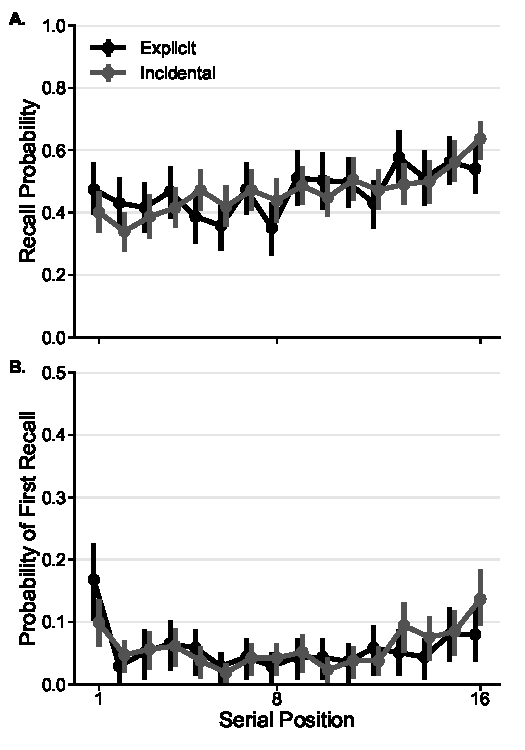
\includegraphics{figures/E2_spc_list1.pdf}
\caption{(A) Serial position curves and (B) probability of first recall curves on the first list under Explicit versus Incidental encoding using the Front Door Task (Experiment 2). \spcpaneltext}
\label{e2_l1_spc}
\end{figure}

\color{black}

Nonetheless, the Front Door Task did not produce a significant TCE on the first list under incidental encoding: Figure~\ref{e2_l1_crp} shows that whereas the Explicit condition \color{red} had a \label{done-11} z(TCE) significantly above zero\color{black}, the Incidental condition showed a flattened lag-CRP and a z(TCE) for which the confidence interval included zero. \color{red} Analyses of the second list, which are reported in the Supplemental Materials for this and subsequent experiments, replicated the Experiment 1 finding of increased contiguity. \color{black}

These results confirm that incidental encoding can \st{eliminate} \color{red} dramatically reduce \color{black} temporal contiguity without substantially decreasing memory performance \citep{NairEtal17}. This lack of coupling between level of recall and level of temporal contiguity has important theoretical implications, which I will consider in the Discussion.

%#####################
%####### E2l1 crp ####
%#####################
\begin{figure}%[hp]
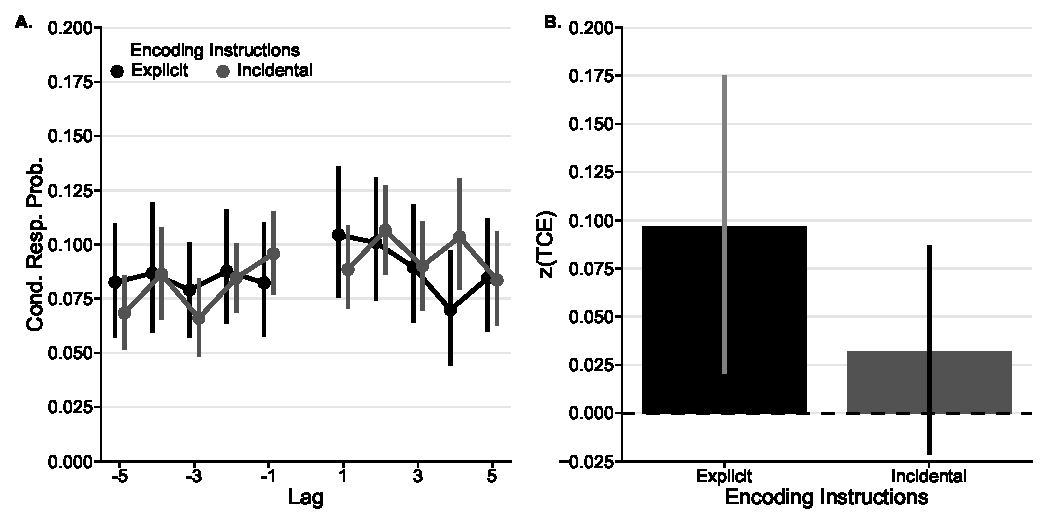
\includegraphics{figures/E2_crp_list1.pdf}
\caption{The temporal contiguity effect (TCE) on the first list under explicit versus incidental encoding using the Front Door Task (Experiment 2). \paneltext}
\label{e2_l1_crp}
\end{figure}




\st{\section{Interim Discussion}}
\st{Experiments 1 and 2 show that the TCE can be absent when intent to encode is absent} \color{red} Experiments 1 and 2 show that when intent to encode is absent, the TCE can be reduced to the point of being statistically indistinguishable from zero\color{black}. This result is consistent with theories that ascribe the TCE to strategic control processes. Under this interpretation, the contiguity-generating processes are more or less inseparable from the intent to encode. But is intent to encode truly necessary to find a TCE? Perhaps not.

\color{red}
Studies showing memory for serial order after incidental learning strongly suggest that participants have access to the temporal information required to produce a TCE \citep{Nair91,Nair90b}.\color{black} \st{An alternate interpretation is that automatic encoding processes do produce contiguity but their effect is obscured by processes required by the judgment task.}  \color{red} Why do they fail to use it? In the final two experiments, I consider two explanations. Experiment 3 tests the possibility that the details of the incidental encoding task determines whether or not temporal contiguity influences memory search. Experiment 4 tests the possibility that temporal information is encoded during incidental learning, but subjects do not automatically use it during memory search unless the memory test requires it.



\section{Experiment 3}
Experiment 3 focuses on the possibility that temporal information is encoded automatically, but its influence is obscured by processes required by the judgment task.\color{black}~For example, many models produce a TCE because the representations of items studied close together are more similar to each other than they are to representations of items studied far apart. The Shoebox and Front Door Tasks encourage subjects to maintain a common mental representation (e.g., image of a shoebox) throughout the list presentation. If this representation is incorporated into the representations of list items, it would increase the similarity of items separated by distant lags, attenuating the TCE. When effortfully memorizing, subjects likely process items in ways that are not necessary for the judgment task, perhaps decreasing the similarity of items separated by distant lags, increasing the TCE. That is, the judgment task might decrease the TCE in a way that is not due to the lack of intent to encode.

More generally, if intentional control processes are required to produce contiguity, it should be challenging, perhaps even impossible, to observe a TCE under incidental encoding. But if control processes simply modulate the effect of automatic contiguity-generating processes (sometimes attenuating the TCE, sometimes accentuating it), it should be easy to find incidental encoding tasks that produce a TCE. Experiment 3 tests these predictions by examining five different encoding tasks.

\section{Method}
The methods were identical to those used in Experiment 2 except for the judgment task instructions (see Table 1 for sample size information).

The question is no longer whether explicit encoding produces a larger TCE than incidental encoding, but rather whether the TCE can ever be observed under incidental encoding. Thus, in Experiment 3, all subjects were given incidental encoding instructions, but were randomly assigned to one of five different judgment tasks that varied in the type of processing required. Otherwise, the methods were identical to those used in Experiments 1 and 2 (see Table 1 for sample size information).

\subsection{Processing Task Manipulation}
In all conditions, subjects were asked to make a judgment about each word as it was presented. Here, I describe the type of processing that each task was intended to discourage (or encourage). Again, to allow for the same yes/no response for each task, subjects were asked to indicate if the judgment was easy to make under the guise of norming the items for a later study. See the Supplemental Materials for the exact task instructions.



\subsubsection{Weight Task} The Weight Task was similar to the size judgment tasks used in the first two experiments except that it asked subjects to compare each item's \emph{weight} to a common referent: a bottle of water. Specifically, they were asked to judge whether each word referred to an object that was heavier than ``a standard bottle of water you'd purchase from a vending machine''. Because weight is not an easily visualizable attribute, the Weight Task might be expected to reduce the likelihood that subjects will maintain the same vivid mental image throughout the list. Thus, it may produce a larger TCE if associating each item with a common mental image tends to attenuate the TCE.

\subsubsection{Animacy Task} The Animacy Task asks subjects whether each item refers to an object that is living or non-living. Like the Shoebox, Front Door, and Weight Tasks, the Animacy Task requires subjects to consider only a single attribute of each item (i.e., animacy status). But unlike the aforementioned tasks, it does not provide a reference object against which to compare each item. Thus, it further reduces the likelihood of maintaining a single vivid image throughout the list.

\subsubsection{Moving Scenario Task} The Moving Scenario Task asks subjects to judge the relevance of each word to a scenario: moving to a foreign land \citep{NairEtal17}. Subjects are likely to maintain some representation of this scenario across items, but because it does not specify any pre-existing dimension, like size or weight, each item may be expected to activate many different attributes, lowering the similarity of mental representations from item to item.

\subsubsection{Movie Task} The instructions for the Movie Task explain that ``when you read a word, it can trigger many different thoughts'' and gives the example of the word baseball triggering a series of thoughts: ``you might have a mental image of a baseball, you might hear the crack of a bat hitting a ball, you might think of related concepts like ballpark, players, and fans...''. It then asks subjects to allow each item ``to activate as many different thoughts as possible. Then use these thoughts to generate a mental movie (like a detailed image of spending an afternoon at a baseball game or what it is like to be a player on a baseball field).'' Subjects then judge whether or not it was easy to form such a mental movie. This tasks removes the requirement to consider each item along the same dimensions and instead encourages subjects to think deeply about the unique attributes of each item, which might be expected to cause very different mental representations to be activated with each successive item, perhaps increasing the TCE \citep[for a different prespective on the influence of item specific processing on the TCE, see][]{McDaEtal11}. 

\subsubsection{Relational Task} The Relational Task is similar to the Movie Task except instead of being asked to make a new mental movie for each item, subjects are asked to ``try to incorporate each new word into your existing mental movie. For example, if the next word was ``owner'', you should allow it to activate many associated thoughts and then incorporate it into your existing ``ballpark'' movie.'' This condition, which is similar to deep encoding strategies free recall subjects often adopt spontaneously \citep{DelaKnow05}, encourages subjects to notice semantic associations between temporally proximate items. As such, it is much like the ``reminding'' process \cite{Hint16} suggested contributes to the TCE \citep[for a similar manipulation see][]{BowClar69}. Thus, this condition should maximize the chance of observing a TCE. 

\section{Results and Discussion}

\color{red}
Table 1 shows overall recall accuracy and Figure~\ref{e3_l1_spc} shows SPCs and PFRs. The most notable difference among the groups was that, whereas the first four tasks produced SPCs and PFRs similar to those of the incidental encoding conditions of the first two experiments, the Relational Task produced a SPC and a PFR that more closely resembles those seen in multi-trial delayed recall. This suggests that the Relational Task successfully mimicked some features of intentional encoding.

%#####################
%####### 3l1 spc ####
%#####################
\begin{figure}
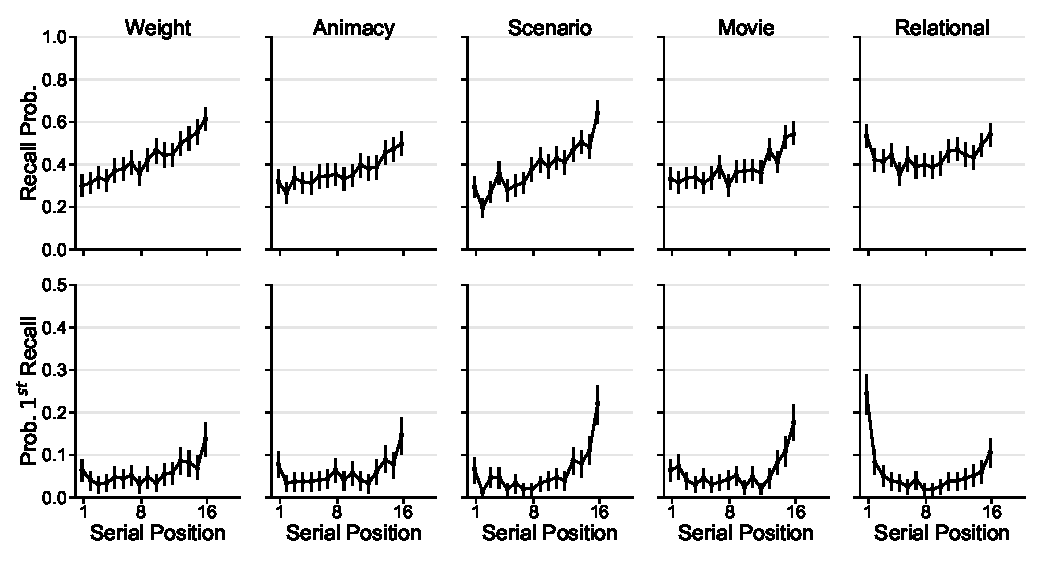
\includegraphics{figures/E3_spc_list1.pdf}
\caption{(Top row) Serial position curves and (Bottom row) probability of first recall curves on the first list under incidental encoding with different judgment tasks (Experiment 3). \spcpaneltext}
\label{e3_l1_spc}
\end{figure}

\color{black}

\st{As seen in Figure 3,}\color{red} Critically,\color{black}~all of the processing tasks produced a TCE under incidental encoding conditions \color{red}(Figure~\ref{e3_l1_crp})\color{black}. For each task, the lag-CRP tends to decrease with increasing $|lag|$ and the z(TCE) is significantly above zero. These results show that although the TCE can be attenuated under incidental conditions (as in Experiments 1 and 2), the lack of intent to encode, per se, does not eliminate contiguity.

Indeed, perhaps the most remarkable feature of the data is how little the size of the TCE differs among the tasks, consistent with the suggestion that the TCE is due to automatic encoding processes. The only condition for which the z(TCE) differed significantly from any other condition was the Relational Task condition, which asked subjects to integrate each item into an ongoing movie.\footnote{The Relational Task also increased recall relative to most of the other tasks (see Table 1), which replicates \citet{BowClar69}} This suggests that encouraging subjects to notice semantic similarities among items does indeed enhance temporal contiguity \citep{Hint16}, at least under incidental encoding conditions.

\st{It is also notable that there is substantial variation in recall levels across conditions (see Table 1) despite modest variation in the TCE, which is consistent with Experiments 1, 2 and Nairne et al. (2017). I return to this point in the General Discussion.}

\st{Finally, we note} \color{red}It should be noted \color{black} that although Experiments 1 and 2 conceptually replicated Nairne et al.'s (2017) finding of no contiguity under incidental encoding using different encoding tasks, Experiment 3 failed to replicate the finding using an encoding task (Moving Scenario Task) almost identical to Nairne et al.'s. \st{This failure may be due to our larger sample size ($n=299$ here versus $N=80$ in E1 and $N=80$ in E2 of Nairne et al.) providing more power to detect a small contiguity effect combined with seemingly minor methodological differences (e.g., different list lengths and presentation rates). In any case,} \color{red}Nonetheless,\color{black}~the message across the present three experiments is consistent with Nairne et al.'s findings: incidental encoding \emph{can} \st{eliminate contiguity and it certainly} reduce the size of the effect relative to explicit encoding \color{red} without substantially reducing recall accuracy\color{black}.

\color{red}
The failure to exactly replicate the Nairne et al. (2017) null finding may be due to a larger sample ($n=299$ here versus $N=80$ in E1 and $N=80$ in E2 of Nairne et al.), providing more power to detect a small contiguity effect. But this raises the possibility that the current Experiments 1 and 2 were underpowered as well. Although sample sizes were selected to provide enough power to detect effects considerably smaller than those typically reported, as discussed above, the observed effects were even smaller than expected. Indeed comparing the significant z(TCE) scores in Figure~\ref{e3_l1_crp} with the non-significant ones in Figures~\ref{e1_l1_crp}~and~\ref{e2_l1_crp}, shows that they all have a similar magnitude---of the 7 incidental encoding conditions reported across the three figures, only the Relational Task condition is significantly different from any other. \label{power}Excluding the Relational Task, the average effect size in Experiment 3 measured by Cohen's $d$ was 0.16. Achieving 95\% power to detect this effect would require 510 participants, considerably more than the sample sizes in Experiments 1 and 2.

Thus, there are (at least) two mutually exclusive interpretations of the findings of Experiment 1--3. First, it could be that only encoding tasks that use a common referent tend to suppress the TCE. Second, it could be the case that a small TCE of approximately equal magnitude is present in all three Experiments but they were not sufficiently powered to detect it reliably. Experiment 4 attempts to distinguish between these interpretations.

  


\color{black}

%#####################
%####### 3l1 crp ####
%#####################
\begin{figure}%[hp]
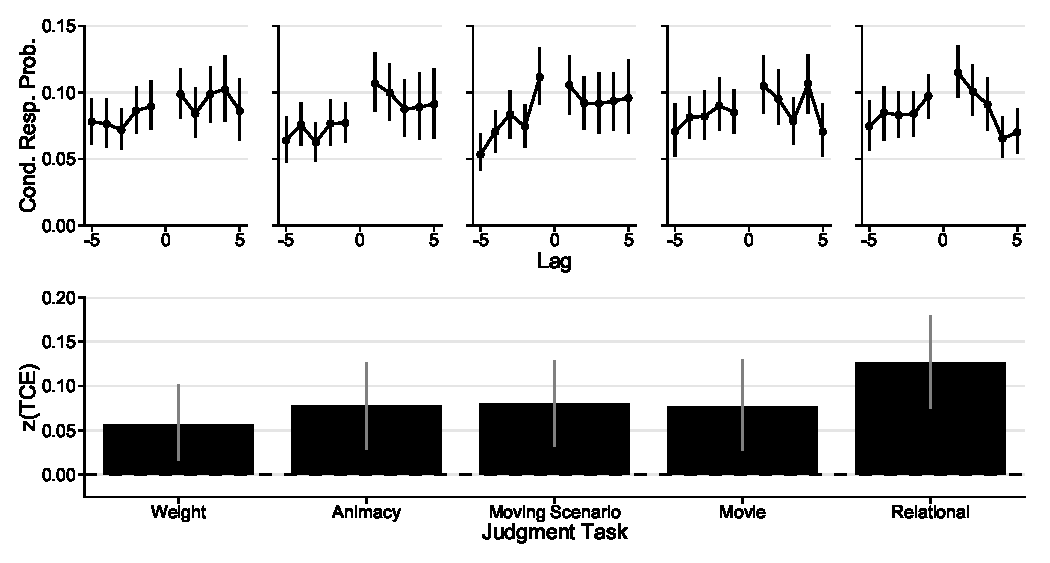
\includegraphics{figures/E3_crp_list1.pdf}
\caption{The temporal contiguity effect (TCE) on the first list under incidental encoding with different judgment tasks (Experiment 3). (Top) Lag-conditional response probability functions. Error bars are bootstrapped within-subject 95\% confidence intervals. (Bottom) The average z(TCE).  Error bars are bootstrapped between-subject 95\% confidence intervals. z(TCE) for a given subject is computed as follows: An observed temporal factor score was computed as the average percentile ranking the temporal lag of each actual transition in the recall sequence with respect to the lags of all transitions that were possible at that time. To determine the temporal factor score expected by chance, a permutation distribution was created by randomly shuffling the order of recalls within the sequence 10,000 times and computing a temporal factor score for each shuffling. The reported value, z(TCE), is z-score of the observed temporal factor score within the permutation distribution.}
\label{e3_l1_crp}
\end{figure}


\color{red}
\section{Experimet 4}
\label{newexp}




% But there are (at least) three possible interpetations of the findings of E1-3. First, it could be that encoding tasks that use a common referent tend to suppress the TCE. Second, it could be the case that a small TCE of approximatel equal magnitude is present across all experiments but the experiments were underpowered. Third, it could be the case that temporal information is encoded in all cases but is simply not sponteniously used by participants during free recall memory search. Experiment 4 attempts to distinguish among these possibilities and to clarify the theoritical implications of this cavet by answering two questions.

Experiment 4 includes three conditions. The first condition is a conceptual replication of the incidental encoding task of Experiment 1 (judge each item's size against the common referent of a shoebox), but with a larger sample size to determine if a residual TCE remains. 

The remaining two conditions were designed to test two different hypotheses.
The first hypothesis was that the TCE is reduced by incidental encoding tasks that require judging each list item against an common referent. This hypothesis was tested by replacing the common referent of "shoebox" with a unique size referent for each list item (e.,g is item 1 larger than a golf ball; is item 2 larger than a penny; is item 3 larger than a piano, etc.). The second hypothesis was that temporal associations generally \emph{are} formed under incidental encoding but that participants do not spontaneously adopt a retrieval strategy that makes use of them. This hypothesis was tested by using the same shoebox size judgment encoding task as the first condition, but replacing the surprise free recall test with a surprise serial recall test. 

\section{Method}
\label{TODO-8}
\subsection{Participants}
For this experiment participants studied and recalled only a single list, which provided extra time for a short demographic questionnaire at the end of the study. To achieve 95\% power, a target sample size of at least 500 participants per condition was set. A total of 1591 individuals participated (see Table 1 for sample sizes and awareness rates by condition), of these there were \males~males, \females~females, \others~transgender individuals, and~\notans~individuals who preferred not to answer. There were \engY~native English speakers, \engN~non-native English speakers, and \engS~individuals who preferred not to answer.  The mean age was \age. The highest level of education attained was less than high school for \noed~ individuals, high school for \hschool, an associates degree for \ass, a masters degree for \mas, an advanced degree (e.g., PhD, MD, JD) for \phd, and \notansed~ preferred not to answer.

Participants were assigned to one of three conditions. All conditions had incidental encoding but varied in the judgment task and how participants were asked to recall the words during the surprise memory test.

\subsubsection{Varying Size--Free Recall}
The Varying Size  was identical to the Shoebox Task from Experiment 1 with three differences. First, instead of judging every word against a common referent (a shoebox), a different referent was randomly selected for each word (see the Supplemental Materials for a full list of referents). Second, instead of deciding if the presented word would ``fit in'' a Shoebox, participants were asked if the word was ``larger than'' the referent to allow for cases where the referent was not a container (e.g., AFRICA: "Is it easy to judge if it is larger than a Golf Ball"). Third, each word was presented for 5 sec (as opposed to the 4 second presentation rate of all other conditions) because the changing referent from item-to-item made the task more complex. Like all previous conditions, the list was followed by a math distractor and a surprise free recall test.


\subsubsection{Constant Size--Free Recall}
The Constant Size task was identical to the Varying size task (including the "larger than" wording of the judgment task and the 5 second presentation rate) with the exception that the size referent was a Shoebox for all items. The list was followed by a math distractor and a surprise free recall test.

\subsubsection{Constant Size--Serial Recall} 
This condition was identical to the Constant Size--Free Recall except that the list was followed by a surprise serial recall task. After the math distractor, participants were given same recall instructions used in the other conditions with one additional sentence: ``Try to recall the words in the ``\textbf{same order you saw them}'' (including the bold emphasis).

\section{Results and Discussion}

The Varying Size--Free Recall free recall condition produced lower overall recall than either of the other two conditions (Figure~\ref{e4_l1_spc}A; Table 1), which is not surprising given the potential for interference between the list items and the varying size referents. Participants in the Constant Size--Serial condition produced an intermediate level of recall and, not surprisingly, showed a higher probability of initiating recall from the first item in the list (Figure~\ref{e4_l1_spc}B). 

\begin{figure}
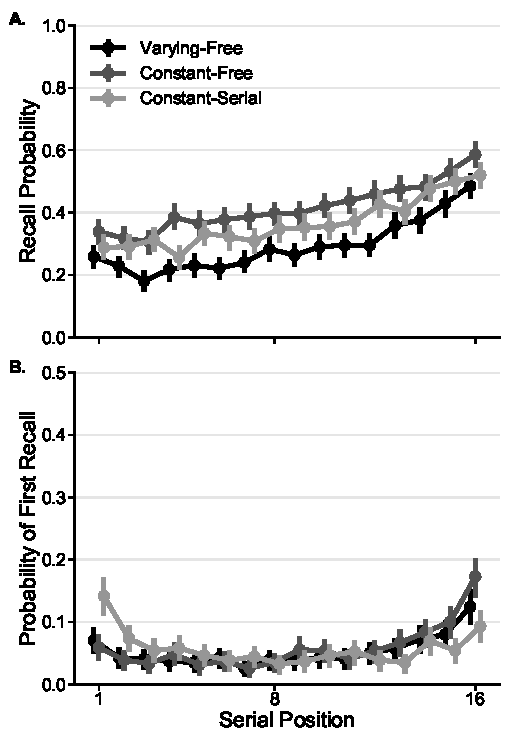
\includegraphics{figures/E4_spc_list1.pdf}
\caption{(A) Serial position curves and (B) probability of first recall curves on the first list as a function of encoding task variability and recall instructions (Experiment 4).\spcpaneltext}
\label{e4_l1_spc}
\end{figure}

Figure~\ref{e4_l1_crp} reveals that all three conditions showed a significant TCE. Moreover, as is clear from the overlapping confidence intervals, the level of the TCE did not differ significantly across conditions. These results point to three important conclusions. 

First, participants in the Constant Size--Free recall condition, which was almost identical to the incidental condition in Experiment 1, encoded temporal information and spontaneously used it to guide memory search during free recall. This suggests that the failure to find a significant TCE in Experiments 1 and 2 may have been due to a lack of statistical power rather than a total absence of a TCE. To be clear, their is no doubt that incidental encoding can reduce the TCE to near zero, which is a very important finding. But, as discussed in detail below, the presence of a small residual TCE is also of considerable theoretical consequence.

Second, changing the size referent of the judgment task from item to item had no effect on the size of the TCE. This suggests that the reduced TCE under incidental encoding is not the result increasing the effective similarity among list items by linking each item to a common context. This conclusion should be tempered, however, by the observation that changing the referent for each item introduces the need for source monitoring (distinguishing list items from size referents during recall), which could potentially impact the TCE.  

Third, explicitly asking subjects to recall the words in serial order, rather than any order they want, did not significantly increase the TCE. This suggests that the reduced TCE after incidental encoding is not entirely due to a failure to adopt a strategy of using temporal information to guide memory search. These data are consistent with the claim that incidental encoding reduces the amount of temporal information available to subjects. Although it possible future work using a different test of order memory might reveal additional latent knowledge of temporal associations. For example, one could encourage subjects to use the order of items to aid recall without asking them to exactly reproduce the serial order. %Or one could reduce the influence of output interference and item memory by presenting a shuffled list of the items during recall and asking subjects to order them \citep[e.g.,][]{NairEtal17}.


\begin{figure}%[hp]
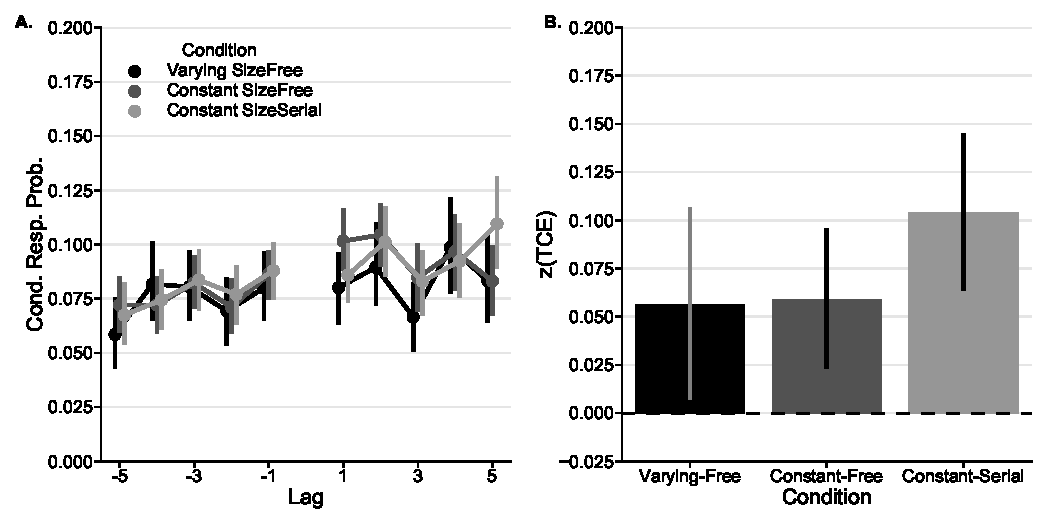
\includegraphics{figures/E4_crp_list1.pdf}
\caption{The temporal contiguity effect (TCE) on the first list as a function of encoding task variability and recall instructions (Experiment 4).\paneltext}
\label{e4_l1_crp}
\end{figure}

\color{black}





\section{General Discussion}
\color{red}
The TCE is the observation that the order in which events are experienced has a powerful influence on the order in which those events are recalled. The current results place an important caveat on this general observation: when the events are experienced without expectation of a memory test, the influence of order of experience on order of recall can be dramatically reduced.  

\label{zerovsnear}
\subsection{Zero or Near Zero?}
The findings of these 4 Experiments adjudicate between two theories of the TCE: Does the TCE depend on control processes that implement task-specific strategies during deliberate encoding \citep{Hint16}? Or does the TCE depend on automatic task-general processes that operate even when we form new memories in the absence of deliberate study \citep{HealKaha17}? The former possibility suggests the TCE should be easily eliminated by removing the impetus to engage controlled processes. The latter suggests the the TCE should be observable under most encoding circumstances. The data tell us that neither view is totally correct.

Taken as a whole, the results show that the TCE is not reliably eliminated by removing the intent to encode. A meta-analysis of the various incidental encoding conditions across the 4 experiments, presented in Figure~\ref{meta}, reveals that the average effect size is significantly above zero. To be conservative, this analysis excludes the Relational condition from Experiment 3 (because it significantly increased the TCE) and the Constant-Serial condition from Experiment 4 (because its serial recall test directly encouraged subjects to use temporal information). Including these two conditions would result in a larger average effect size. Among the included conditions none had an effect size that was significantly different from any other. In other words, although individual conditions may not have sufficient power to detect an effect, across conditions there is very strong evidence for a small but robust incidental TCE. This is a case where a small effect is an important effect as it provides as existence proof for temporal contiguity under incidental encoding and rules out the possibility that the TCE is an artifact of task-specific strategies. 

\begin{figure}%[hp]
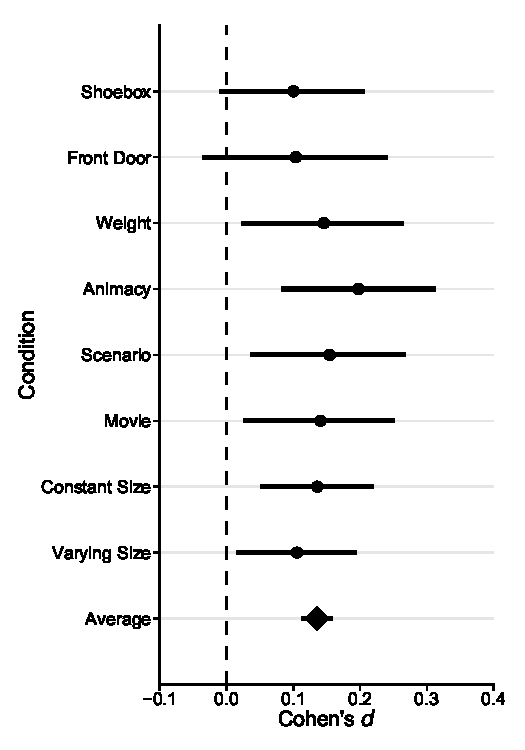
\includegraphics{figures/meta.pdf}
\caption{Forest plot of the effect size, Cohen's $d$, of the TCE in 8 different conditions in which incidental encoding was followed by a free recall task along with the average effect size across the conditions. The Relational condition from Experiment 3 was excluded because it significantly increased the size of the TCE and its inclusion would inflate the estimate of the average effect size. The Constant-Serial condition from Experiment 4 was excluded because it used a serial recall test rather than a free recall test. Error bars on the individual conditions are bootstrapped 95\% confidence intervals; the error bar on the average is the 95\% confidence interval computed by multiplying the standard error of mean of the 8 condition means by $t_{8-1}=2.365$.}
\label{meta}
\end{figure}


\subsection{Implications for Theories of Episodic Memory}
Although these results strongly suggest that the TCE arises from automatic encoding processes, they just as clearly suggest that we do not yet adequately understand these processes.

For example, under the Retrieved Context family of models \citep[e.g.,][]{PolyEtal09,LohnEtal14,HealKaha15}, which arguably provide the most comprehensive theory of TCE, the mechanisms that produce contiguity are inexorably linked to those that encode memories in a way that makes it difficult to decouple accurate recall and from a large TCE. These models assume that episodic memory for an event is formed by associating list items with the current state of a context representation that changes across time. This same context representation is then used as a retrieval cue which naturally encourages memory search to focus on events that occurred near each other in time. Because a small residual TCE remained, the current data do not falsify these models, but they do set a serious challenge for modelers: How can these models account for near zero levels of contiguity in the face high recall accuracy? In other words, how can context provide an effective retrieval cue for some items, and thus produce high levels of recall, without simultaneously providing an effective cue for temporally adjacent items?

This issue is illustrated in Figure~\ref{corr} which plots level of recall versus the level of the TCE across all 12 conditions presented in this manuscript. The correlation is quite small and non-significant \color{black} suggesting that recall success may depend less on temporal contiguity than has been suggested by analyses of individual differences in free recall of explicitly encoded lists \citep{SedeEtal10,HealEtal14}. Indeed, some of the conditions with the highest recall levels had the lowest levels of contiguity. Again, this finding does not falsify the models, but it does challenge them. 

The precise nature of the relationship between time and context drift in these models points to one possible answer to this challenge. Although the change in context from time $t$ to time $t+lag$ is correlated with the passage of time, it is not \emph{driven} by time in most Retrieved Context models \citep[but see][for a model in which drift is driven by time]{HowaEtal14a}. Instead, context drift is driven by the cognitive representations activated by external and internal events. As a result, the similarity of the context representation, $\mathbf{c}_t$, at time $t$ to the context representation at some other time, $\mathbf{c}_{t+lag}$, is partly a function of the similarity of the cognitive representations activated by the events that intervene between $t$ and $t+lag$. 

Under some incidental encoding tasks, the cognitive representations activated by successive items are likely to be similar, causing context to drift slowly and resulting in a shallow\color{red}, perhaps near zero,\color{black}~contiguity effect. By contrast, if subjects are intending to encode items for a memory test they are likely to engage in elaborative processing which might cause context to drift rapidly and produce a steeper contiguity effect. The current Experiment 4 attempted to manipulate this drift rate experimentally and found no evidence that it increased the TCE, though other methods of manipulating context drift \citep[e.g.,][]{PolyEtal12} might yield different results. A critical question for modelers then, is whether existing models can use differential drift rates to capture the large difference in TCE between Incidental and Explicit conditions while simultaneously capturing the near equal levels of recall.

But even if existing models can fit the difference between explicit and incidental encoding by fine-tuning model parameters, we are still left with a large gap in our understanding of how encoding processes influence contiguity. How does the memory system accomplish this fine-tuning over the course of a single list without the benefit of a modeler's fitting algorithms? Some control process must rapidly translate task instructions into a ad hoc parameterization of task-general memory mechanisms that is tailored to the task demands \cite{HealEtal14,AtkiShif68}. There have been few attempts to model how automatic memory processes interact with controlled processes to meet task demands \citep{LehmMalm13,PolyEtal09}. The challenge is avoiding adding a homunculus to the models that does the hard work of translating task instructions into encoding processes.

\begin{figure}%[hp]
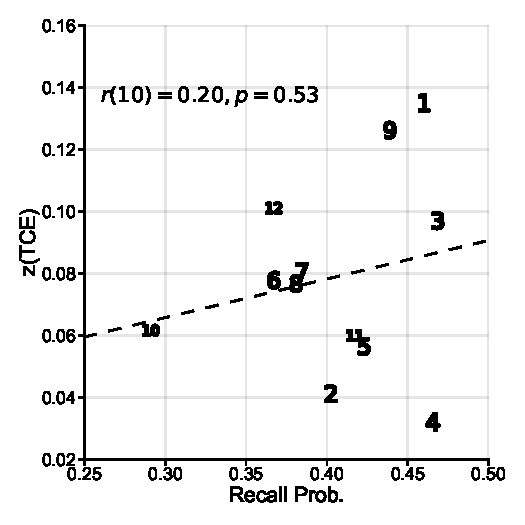
\includegraphics{figures/correlation.pdf}
\caption{The size of the temporal contiguity effect versus the overall level of recall. Each dot represents the average of one of the conditions 12 conditions reported across the 4 experiments: 1 = E1 Explicit; 2 = E1 Incidental; 3 = E2 Explicit; 4 = E2 Incidental; 5 = E3 Weight; 6 = E3 Animacy; 7 = E3 Moving Scenario; 8 = E3 Movie; 9 = E3 Relational; 10 = E4 Varying-Free; 11 = E4 Constant-Free; 12 = E4 Constant-Serial.}
\label{corr}
\end{figure}

\color{black}


\subsection{Conclusion}
In summary, these results show that control processes are not necessary to produce a TCE, but that they can powerfully influence the size of the effect and nearly eliminate it. Thus, the results point to serious limitations in existing theories of TCE---we understand much about how memory encoding processes produce temporal contiguity, but we understand little about how these processes are controlled.

\bibliography{healey_lab}
\end{document}